\documentclass[
	letterpaper, % Paper size, specify a4paper (A4) or letterpaper (US letter)
	10pt, % Default font size, specify 10pt, 11pt or 12pt
]{CSUniSchoolLabReport}

%----------------------------------------------------------------------------------------
%	REPORT INFORMATION
%----------------------------------------------------------------------------------------

\title{Linked Lists and the \texttt{gdb} Debugger\\ Embedded Design: Enabling Robotics \\ EECE2160} % Report title

\author{Michael \textsc{Brodskiy}\\ \small \href{mailto:Brodskiy.M@Northeastern.edu}{Brodskiy.M@Northeastern.edu}}

\date{March 30, 2023} % Date of the report

%----------------------------------------------------------------------------------------


\begin{document}

\maketitle % Insert the title, author and date using the information specified above

\begin{center}
	\begin{tabular}{l r}
		Date Performed: & March 23, 2023 \\ % Date the experiment was performed
        Partner: & Dylan \textsc{Powers} \\ % Partner names
		Instructor: & Professor \textsc{Shazli} % Instructor/supervisor
	\end{tabular}
\end{center}

\newpage

\begin{abstract}

  The purpose of this laboratory experiment was to work with classes and familiarize oneself with the linked list advanced data structure, as well as further experience with pointers and memory addresses and their respective operators. By generating a program to interface with a linked list containing a fabricated class, while at the same time avoiding segmentation faults, a stronger grasp of these concepts was created. To avoid segmentation faults, the \texttt{gdb} debugger was employed.

\end{abstract}

\begin{flushleft}

  \textsc{Keywords:} \underline{Linked list}, \underline{class}, \underline{pointer}, \underline{memory address}, \underline{segmentation fault}, \underline{\texttt{gdb}}

\end{flushleft}

\newpage

\section{Equipment}

\hspace{.5 in} Available equipment included:\\

\begin{itemize}

  \item DE1-SoC board

  \item DE1-SoC Power Cable

  \item USB-A to USB-B Cable

  \item Computer

  \item MobaXTerm SSH Terminal

  \item USB-to-ethernet Adapter

\end{itemize}

\section{Introduction}

In general, a debugger tool is used to inspect the memory of a program in a controlled execution environment, with the common objective of identifying the presence of bugs in a program. In this lab, one goal was to use the \texttt{gdb} bugger to debug programs through step-by-step execution and memory inspection. Along with this goal, this lab had a secondary goal to use linked lists as an alternative data structure to store sequence elements, where insertion and deletions have a constant cost. Then, after using both these skills separately, the lab combines them with the purpose of using the \texttt{gdb} debugger to explore the execution of a main program using linked lists.

\section{Discussion \& Analysis} 

\subsection{Pre-lab}

\begin{figure}[H]
  \centering
  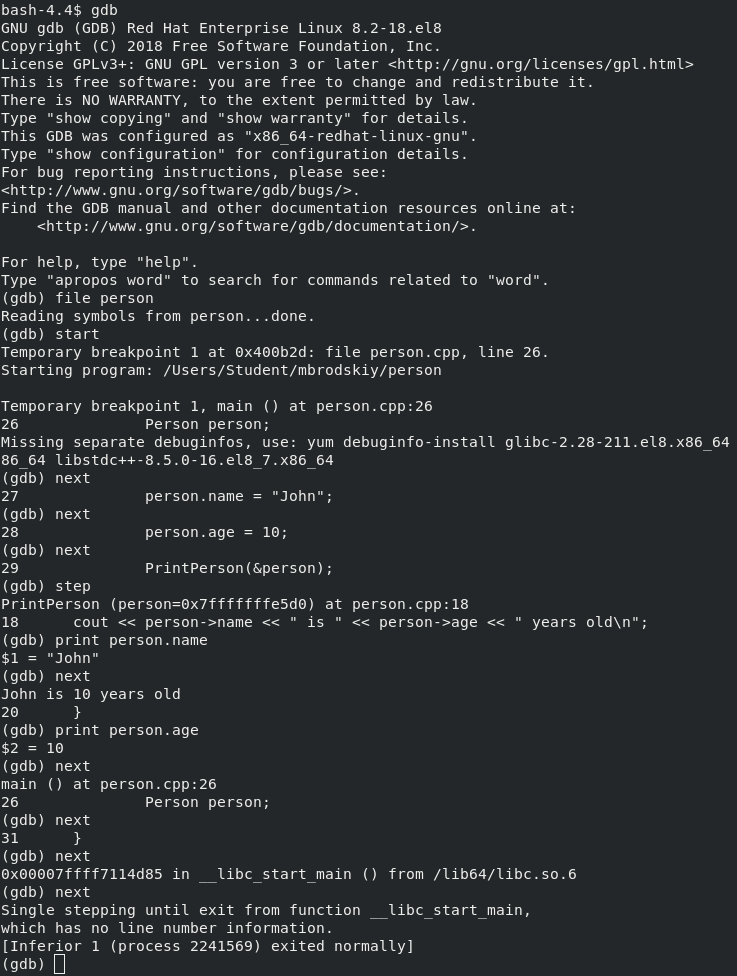
\includegraphics[width=.7\textwidth]{Figures/gdb.png}
  \caption{\texttt{gdb} output}
  \label{fig:1}
\end{figure}

The \texttt{gdb} commands may be explained as follows:

\begin{itemize}

  \item \texttt{file person} selects the binary called person as the file for analysis

  \item \texttt{start} begins analysis of ``person''

  \item \texttt{next} moves to the next point of interest

  \item \texttt{step} enters the function at the current line

  \item \texttt{print} prints the known information for a certain, specified value

\end{itemize}

\lstinputlisting[
    caption=Menu Printing Code, % Caption above the listing
    label=lst:L1, % Label for referencing this listing
    language=C++, % Use C++ functions/syntax highlighting
    frame=single, % Frame around the code listing
    showstringspaces=false, % Don't put marks in string spaces
    numbers=left, % Line numbers on left
    numberstyle=\tiny, % Line numbers styling
    backgroundcolor=\color{black!5}, % Set background color
    keywordstyle=\color{magenta!80}, % Set keyword color
    commentstyle=\color{blue!80}, % Set comment color
    stringstyle=\color{green!80}, % Set string color
    breaklines=true
  ]{Code/PreLab.cpp}

\begin{figure}[H]
  \centering
  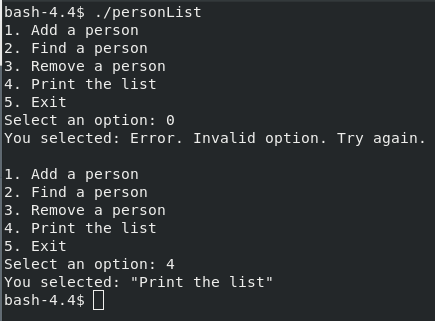
\includegraphics[width=.9\textwidth]{Figures/output.png}
  \caption{Sample menu output}
  \label{fig:2}
\end{figure}

\subsection{Assignment 1}

The goal of Assignment 1 was to load a program \texttt{person} on \texttt{gbd} and set a breakpoint at the beginning of the function \texttt{PrintPerson}. In Figure \ref{fig:3}, the output is provided for the commands (\texttt{gdb}) \texttt{print person}, (\texttt{gdb}) \texttt{*person}, (\texttt{gdb}) \texttt{print->name}, and (\texttt{gdb}) \texttt{print->age}.

\begin{figure}[H]
  \centering
  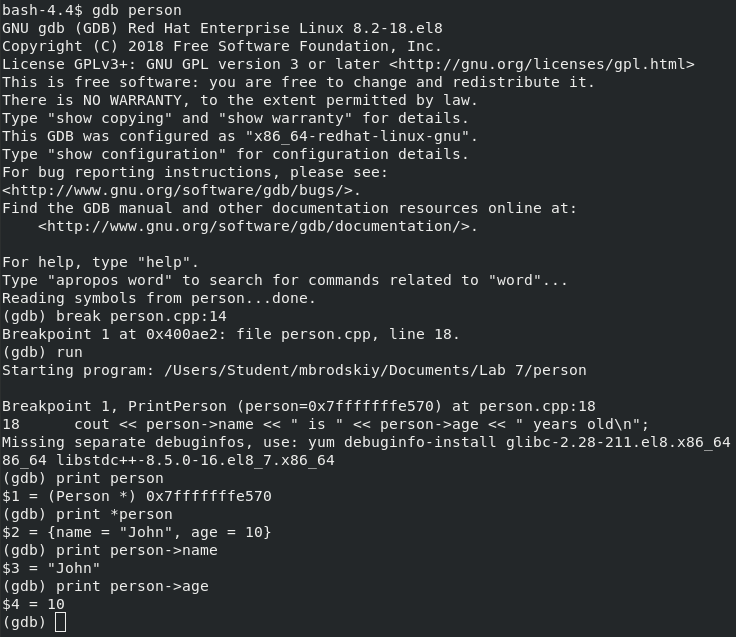
\includegraphics[width=.9\textwidth]{Figures/Assign1.png}
  \caption{Output given by \texttt{gdb} for specified commands}
  \label{fig:3}
\end{figure}

In the output shown it can be seen that the first command (\texttt{gdb}) \texttt{print person} prints the value of the person variable which is a pointer to a \texttt{Person} object. The value of \texttt{person} is \texttt{0x7fffffffe570}. The next command, (\text{gdb}) \texttt{print *person}, prints the contents of the \texttt{Person} object that \texttt{person} is pointing to. The output shows that there is a name attribute of “John” and an age attribute of 10. As for the third command, (\texttt{gdb}) \texttt{print person->name} the program is requesting the value of the name attribute of the \texttt{Person} object which is John as shown. Lastly, (\texttt{gdb}) \texttt{print person->age} prints the value of the age attribute of the \texttt{Person} object. This is why 10 is out after this command is displayed. 

\subsection{Assignment 2}

The goal of Assignment 2 was to start with the implementation of a main program to test the linked list, with a similar structure to the one used to test the dynamically growing array in the previous lab. To do this, a program was written that includes all the type definitions and functions presented in class to manage the \texttt{List} and \texttt{Person} data structures, together with an implementation of the main program. The complete code of the program is included in the entire program, included in the Appendix below.

\subsection{Assignment 3}

The purpose of Assignment 3 was to run the program written in Assignment 2 several times in order to test the behavior of each menu option. For each option, the output of the program is shown below.

\begin{figure}[H]
  \centering
  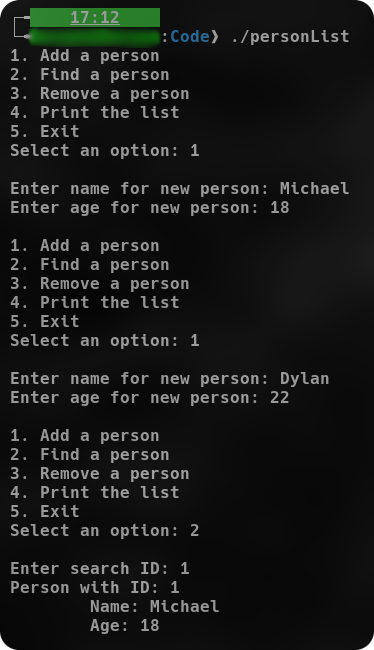
\includegraphics[width=.6\textwidth]{Figures/Assign3.png}
  \caption{Shows menu options 1 and 2}
  \label{fig:4}
\end{figure}

Figure \ref{fig:4} shows the first menu option twice. Option 1 is selected and the name Michael and the age 18 are entered and stored. Then, Option 1 is selected again and the name Dylan and the age 22 are entered and stored. Finally, Option 2, Find a person, is selected and the search ID of 1 is entered. With this information, the program outputted the name Michael and the age 18. This output tells the user that the name Michael and the age 18 were successfully added and that it is possible to locate the name and age of a person with an id. It makes sense that search id 1 returned Michael and not Dylan, because Michael was entered first. 

\begin{figure}[H]
  \centering
  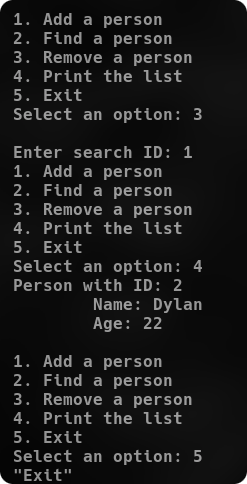
\includegraphics{Figures/Assign3-2.png}
  \caption{Shows menu option 3, 4, and 5}
  \label{fig:5}
\end{figure}

In Figure \ref{fig:5}, Option 3 is shown first. When option 3 was selected, the search id of the person that was to be removed was entered. As can be seen the search id 1 was entered. Next for Option 4, Print the list, this was selected after option 3. Thus, the list should print with only Dylan because Michael was removed, which is what the program returned. Lastly, Option 5, Exit, was selected and the program outputted the message “Exit” and the menu was not displayed again. 

\subsection{Assignment 4}

The goal of Assignment 4 was to run the linked list main program developed in the first part of the lab and set a breakpoint at the end of the loop in function \texttt{main()}, right before the menu is printed for the second time. When the program was run and the menu option that allows the user to insert a new element was selected, the commands (\texttt{gdb}) \texttt{print list}, (\texttt{gdb}) \texttt{print list.head}, and (\texttt{gdb}) \texttt{print list.head->next} were run. The full sequence ran on gdb as well as the output of the commands are shown in Figures \ref{fig:6} and \ref{fig:7}.

\begin{figure}[H]
  \centering
  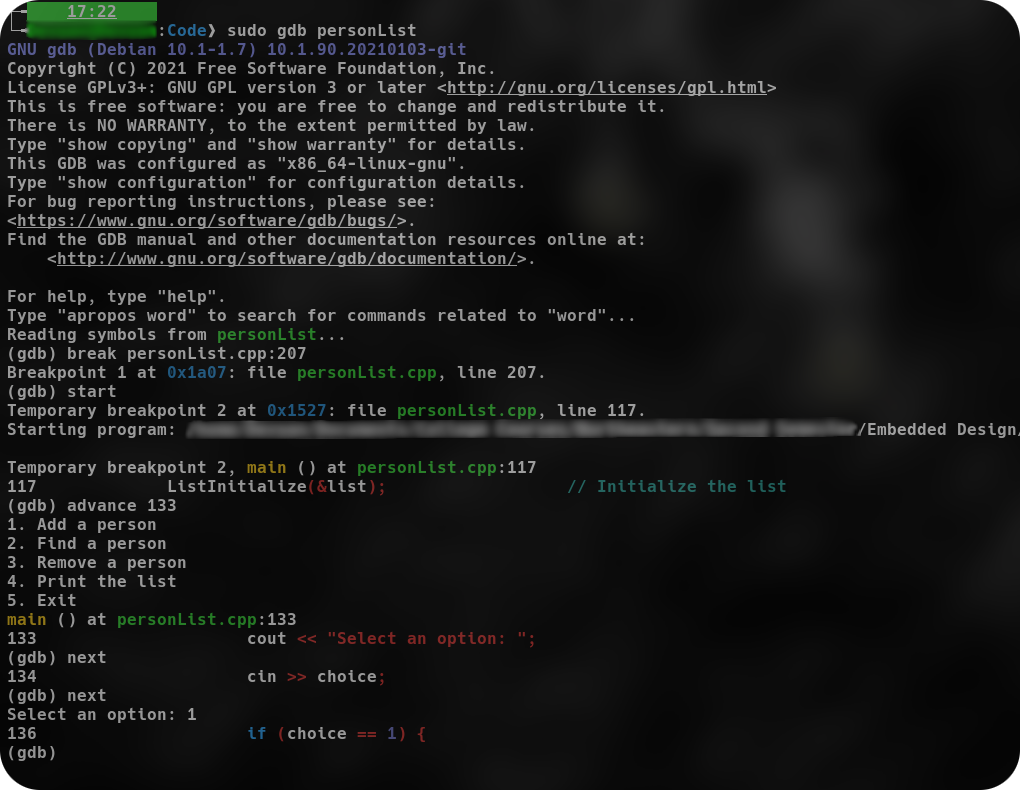
\includegraphics[width=.9\textwidth]{Figures/Assign4.png}
  \caption{First half of full sequence ran on \texttt{gdb} and output of commands}
  \label{fig:6}
\end{figure}

\begin{figure}[H]
  \centering
  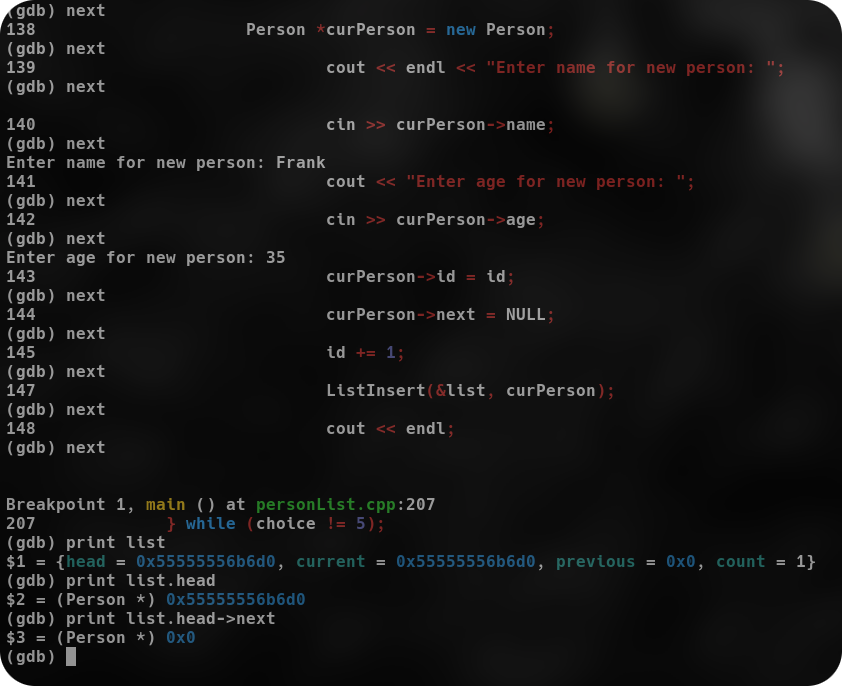
\includegraphics[width=.9\textwidth]{Figures/Assign4-2.png}
  \caption{Second half of full sequence ran on \texttt{gdb} and output of commands}
  \label{fig:7}
\end{figure}

Figure \ref{fig:6} is most of the sequence leading up to running the commands which is shown in Figure \ref{fig:7}. The first of the specified commands run was the \texttt{print list} command. This command printed the current \texttt{Person} object of the linked list. The next command that was run was print \texttt{list.head}. This command outputs the contents of the head field of the starting address. Lastly the print \texttt{list.head->next} command was run, which outputs the next field of the object pointed to by the head. In the case displayed above, the next field was \texttt{NULL} which is why the output was \texttt{0x0}.

\subsection{Assignment 5}

The goal of Assignment 5 was to modify any position of the code in the linked list to strategically make it perform an invalid memory operation that makes the program produce a segmentation fault or to use a real intermediate unstable version of the code that produced a program crash during the development of previous assignments. The program written to do this was run on \texttt{gdb} and the sequence of \texttt{gdb} commands that were run to infer the value of the variable causing the problem is shown in Figure \ref{fig:8}. 

\begin{figure}[H]
  \centering
  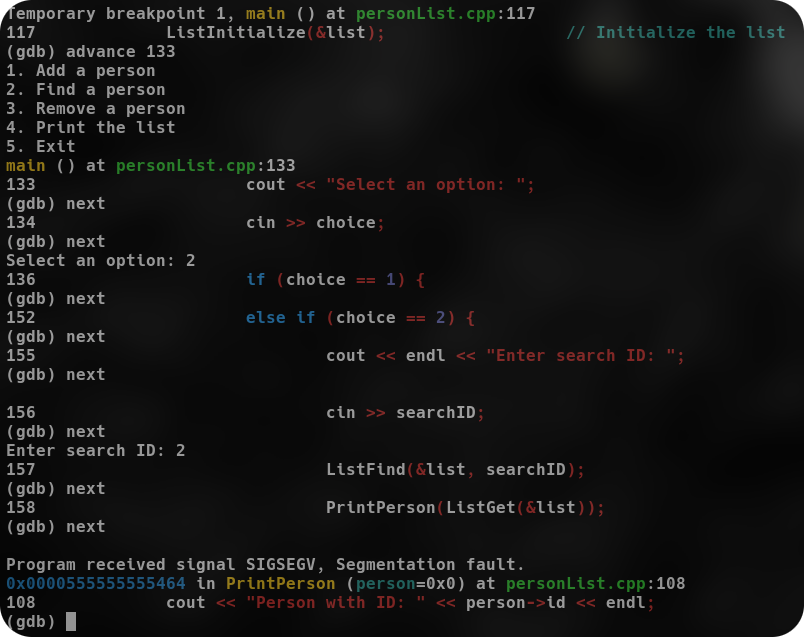
\includegraphics[width=.9\textwidth]{Figures/Assign5.png}
  \caption{Sequence of \texttt{gdb} commands to infer the value of the variable causing the problem}
  \label{fig:8}
\end{figure}

As can be seen in Figure \ref{fig:8}, the (\texttt{gdb}) \texttt{next} command was run until the program received signal SIGSEGV and there was a Segmentation fault. This fault was intentionally produced by permitting the \texttt{ListGet()} function to attempt to access an nonexistent object.

\subsection{Extra Credit}

The extra credit section relied on the creation of a method to sort the linked list in two ways: by person name or by age. In our case, this was done by copying the \texttt{Person} objects over to two parallel arrays, which were then sorted. The existing linked list was then wiped. Subsequently, the now-sorted arrays were inserted back into the linked list. The linked lists were sorted in descending order, as a sorting key was not provided. Below are images depicting a test case of the sorting program.

\begin{figure}[H]
  \centering
  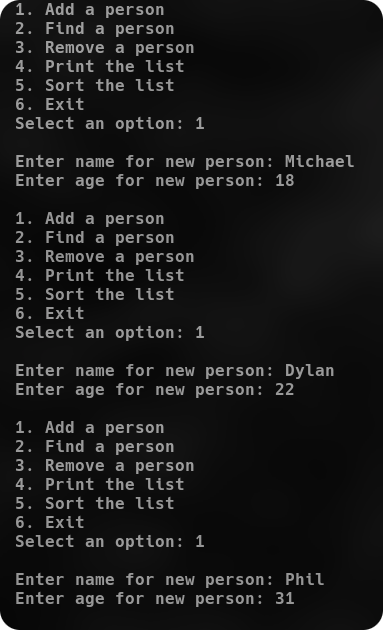
\includegraphics[width=.9\textwidth]{Figures/EC1.png}
  \caption{Extra Credit Test Run, part 1}
  \label{fig:1}
\end{figure}

\begin{figure}[H]
  \centering
  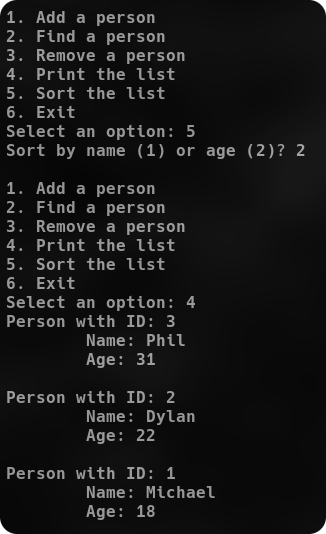
\includegraphics[width=.9\textwidth]{Figures/EC2.png}
  \caption{Extra Credit Test Run, part 2}
  \label{fig:2}
\end{figure}

\begin{figure}[H]
  \centering
  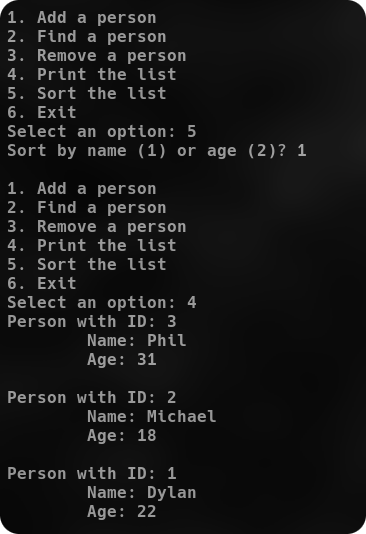
\includegraphics[width=.9\textwidth]{Figures/EC3.png}
  \caption{Extra Credit Test Run, part 3}
  \label{fig:3}
\end{figure}

\section{Conclusion}

Overall, due to the heavy reliance on knowledge of pointers, memory address references, linked lists, class structures, and the ability to interface with the aforementioned, the lab provided an effectively advanced lesson regarding these concepts. Especially in terms of linked lists, working with them in an actual example allowed for a deeper understanding.

\section{Appendix}

\lstinputlisting[
    caption=Complete Source Code, % Caption above the listing
    label=lst:L6, % Label for referencing this listing
    language=C++, % Use C++ functions/syntax highlighting
    frame=single, % Frame around the code listing
    showstringspaces=false, % Don't put marks in string spaces
    numbers=left, % Line numbers on left
    numberstyle=\tiny, % Line numbers styling
    backgroundcolor=\color{black!5}, % Set background color
    keywordstyle=\color{magenta!80}, % Set keyword color
    commentstyle=\color{blue!80}, % Set comment color
    stringstyle=\color{green!80}, % Set string color
    breaklines=true
  ]{Code/personList.cpp}

\end{document}
